\section{Обзор литературы}
\label{sec:lit_review}

\subsection{Обзор существующих аналогов}
\label{sub:lit_review:analogues}
Разработанная в ходе дипломного проектировании система функционального контроля технических средств не имеет широко
известных прямых аналогов. Отсутствие конкурирующих систем вызвано тем следующими причинами:
\begin{itemize}
	\item технические средства, предназначенные для нужд армии имеют ограниченное распространение
	\item протоколы обмена данными между техническими средствами и ЭВМ зачастую являются закрытыми
	\item модуль функционального контроля зачастую является частью закрытого проприетарного ПО, используемого для
		автоматизации задач личного состава
	\item разнообразие устройств, протоколов обмена
\end{itemize}

Таким образом, ввиду невозможности поиска аналогов среди ПО для вооруженных сил, в данном разделе будут проанализированы
наиболее близкие аналоги из других областей.

Наиболее приближенным аналогом является система функционального применяемая на железных дорогах Российской федерации
~\cite{rus_rails}.

\begin{figure}[ht]
	\centering
	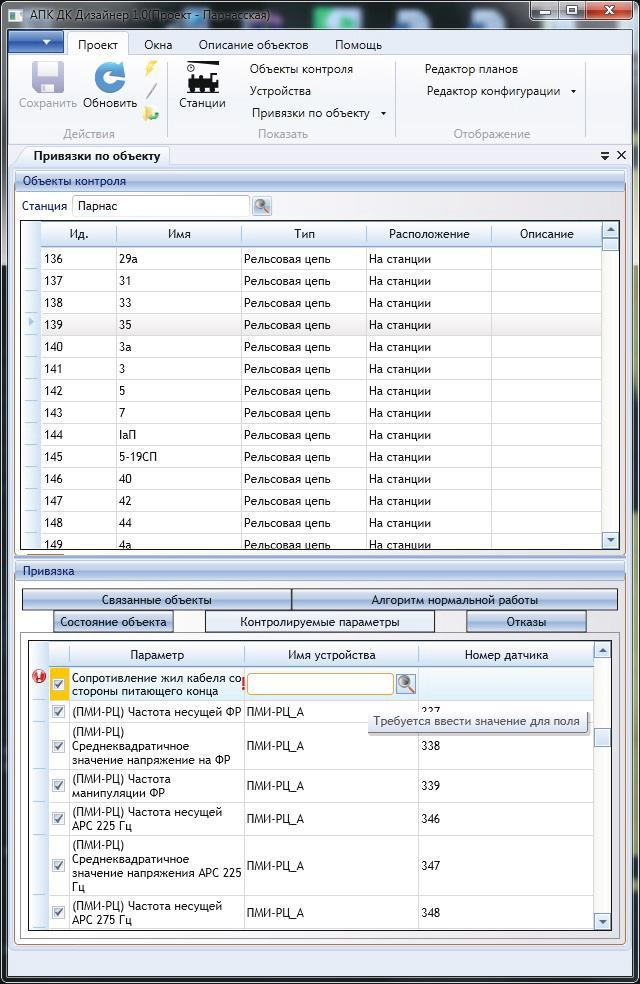
\includegraphics[scale=0.36]{rw_control}
	\caption{Модуль функционального контроля системы автоматизации РЖД~\cite{rus_rails}}
	\label{fig:lit_reiview:analogues:rw_control}
\end{figure}

Данная система функционального контроля позволяет проводить мониторинг различных участков железной дороги, оказывать
управляющие воздействия на объекты контроля, выводить информацию на экран или бумажный носитель, экспортировать данные в
другие программы для работы с результатами мониторинга.

Основные достоинства программы:
\begin{itemize}
	\item удобный интерфейс(использована аналогия с действующими устройствами ввода-вывода информации в
		железнодорожной автоматике и телемеханике(ЖАТ))
	\item вывод информации в иерархическом виде
	\item возможность вывода разного набора информации пользователям в зависимости от должности владельца ПК
\end{itemize}

К недостаткам можно отнести закрытость ПО, отсутствие кроссплатформенности(поддерживается только ОС Windows).

Еще один аналог -- система функционального контроля электронной аппаратуры AX518~\cite{AX518}. Система предназначена для тестирования полупроводниковых микросхем, процессоров, ЦАП, АЦП, устройств в системе радио-идентификации, устройств поддерживающих технологии широкополосного вещания и беспроводных сетей, приемопередатчиков.
Имеется возможность для проведения измерений, как в частотной, так и во временной области, спектрального анализа, измерения RF мощностей, потерь, и шумов.

Система для автоматического тестирования электронных устройств AX518 состоит из 5-слотового шасси стандарта AXIe и 18-слотового шасси стандарта PXI.
Система дополняется компьютером и программным обеспечением.
В состав программного обеспечения входят стандартные библиотеки и специфические программы для тестирования определенных устройств.

Недостатком данной системы является то, что она является аппаратно-программной. Это затрудняет ее внедрение и
значительно повышает стоимость системы.

\begin{figure}[ht]
	\centering
	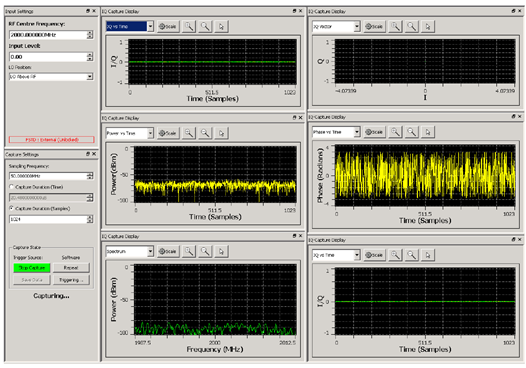
\includegraphics[scale=1.0]{ax518_soft}
	\caption{Программный модуль системы тестирования электронных устройств AX518~\cite{AX518}}
	\label{fig:lit_reiview:analogues:ax518_soft}
\end{figure}

\subsection{Аналитический обзор}
\label{sub:lit_review:analitics}
Технические средства(ТС) --  изделия, оборудование, аппаратура и их составные части, функционирующие на основании законов электротехники, радиотехники и электроники и содержащие электронные компоненты и схемы.

КМУ -- комплекс машин управления.
В состав комплекса машин управления огнем входят:
\begin{itemize}
	\item машина управления командира дивизиона~\cite{div_car}
	\item командно-штабная машина дивизиона
	\item машина управления командира батареи
	\item машина управления старшего офицера батареи
\end{itemize}

\begin{figure}[ht]
	\centering
	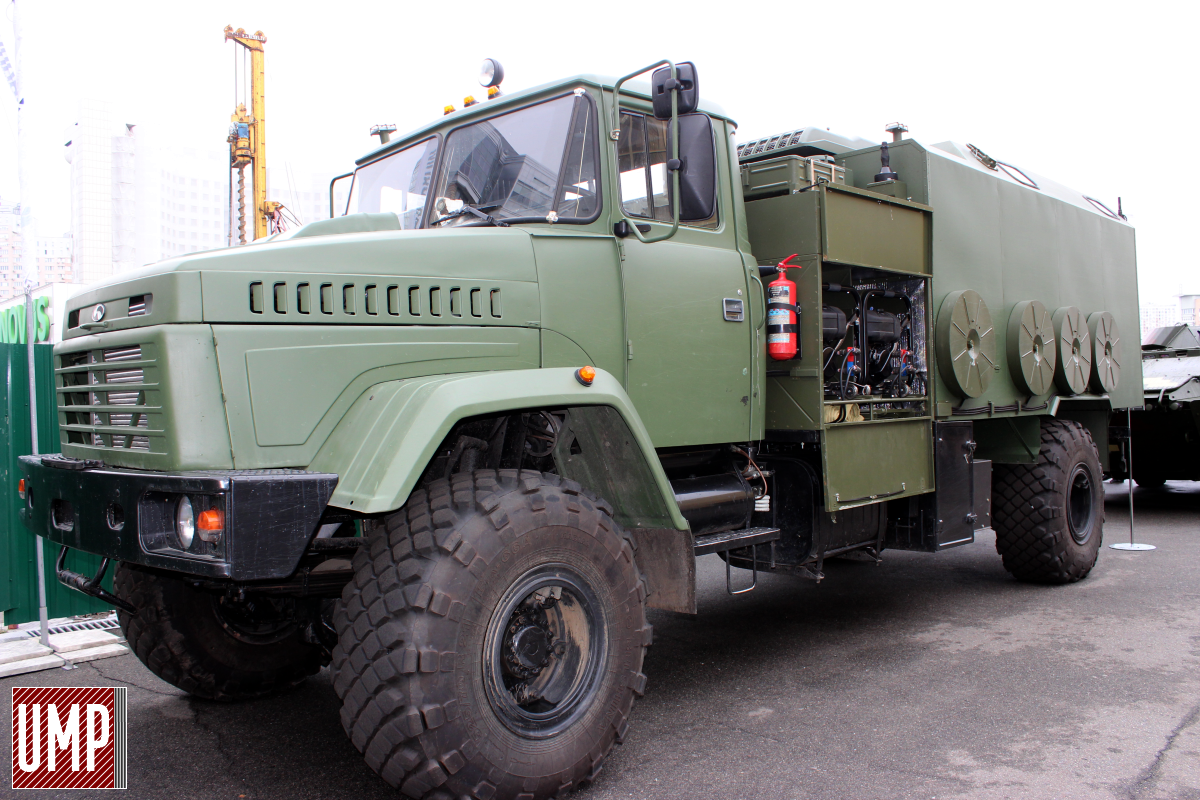
\includegraphics[scale=0.33]{div_com}
	\caption{Машина начальника штаба дивизиона на колесном шасси~\cite{div_car}}
	\label{fig:lit_reiview:analytics:div_com}
\end{figure}
В одном дивизионе имеется несколько машин разного уровня управления, содержащих в своем составе разные ТС.
Например, метеокомплект стоит только на нескольких машинах, радиостанции имеются в каждой машине, бесплатформенная
инерциальная навигационная система(БИНС) присутствует также на каждой машине, но имеют разные типы устройства, локальная вычислительная сеть(ЛВС) присутствует в каждой машине.
Программное обеспечение написано для всех машин КМУ с возможностью выборки подключенных ТС.

Разработанное в ходе дипломного проектирования программное обеспечение предназначено для развертывания в подвижном
комплексе средств автоматизации управления~\cite{patent_2263960}.
Этот подвижный комплекс средств автоматизации управления, размещенный в подвижном объекте на шасси автомобиля повышенной
грузоподъемности, содержит несколько автоматизированных рабочих места(АРМ) должностных лиц, размещенных в кузове-фургоне
подвижного объекта, оборудованных средствами вычислительной техники и средствами передачи данных, радиорелейную станцию
с антеннами, коротковолновую (KB) радиостанцию, две ультракоротковолновые (УКВ) радиостанции, локальную вычислительную
сеть (ЛВС), специальный принтер.

\begin{figure}[ht]
	\centering
	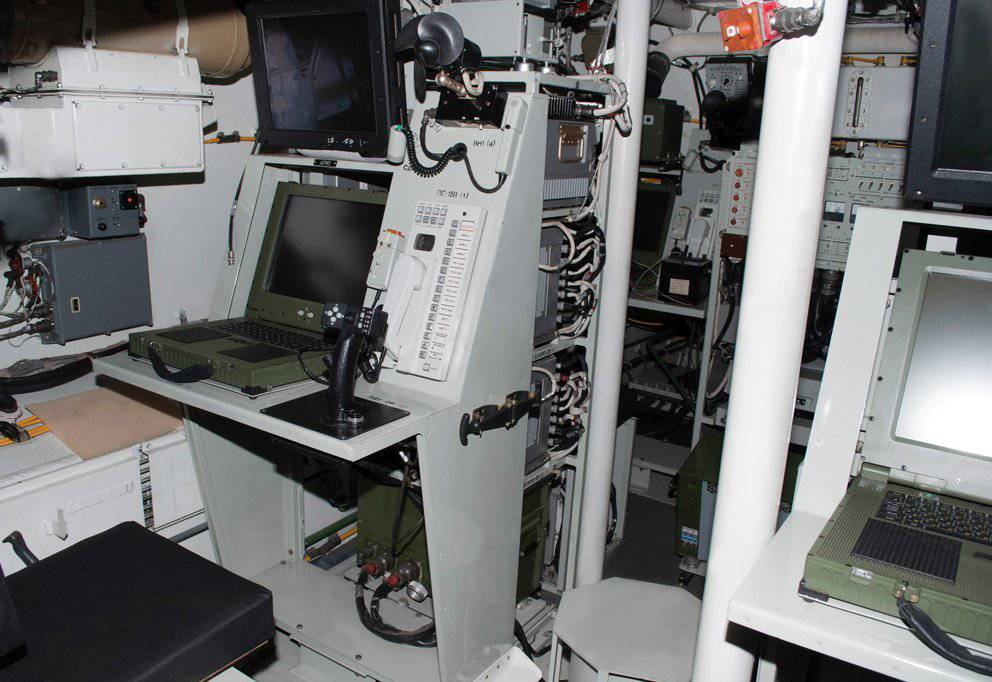
\includegraphics[scale=0.40]{arm}
	\caption{Автоматизированное рабочее место~\cite{patent_2263960}}
	\label{fig:lit_reiview:analytics:arm}
\end{figure}

Программа функционального контроля предназначена для осуществления автоматизации процессов проведения тестирования
технических\break средств.
Программа функционального контроля обеспечивает выполнение следующих функций:
\begin{enumerate}
\item тестирование средств автоматизации, локальной вычислительной сети(ЛВС), визуализацию информации о доступных в ЛВС автоматизированных рабочих местах(АРМ);
\item тестирование и настройку средств связи;
\item тестирование и настройку средств измерения.
\end{enumerate}

\subsection{Интегрированный навигационно-информационный комплекс}
\label{sub:lit_review:ins}

Интегрированный навигационно-информационный комплекс это комплексная бесплатформенная система ориентации и навигации,
построенная с использованием высокоточных акселерометров и волоконно-оптических гироскопов с замкнутым контуром,
построена на принципе комплексирования данных бесплатформенной инерциальной системы (БИНС~\cite{bins500}) с одометром, приемником спутниковых навигационных сигналов (СНС)\break GPS/GLONASS и приемником барометрического давления.
ИНИК имеет модульную систему, которая позволяет получить различные варианты системы, наиболее полно удовлетворяющие потребности по точности измерений, удобству размещения на объекте.

\begin{figure}[ht]
	\centering
	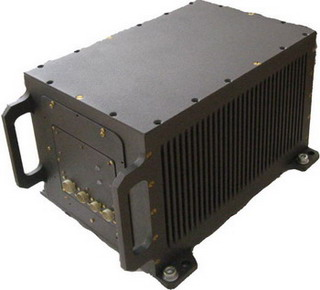
\includegraphics[scale=1.0]{bins}
	\caption{Бесплатформенная инерциальная навигационная система БИНС-500НС~\cite{bins500}}
	\label{fig:lit_reiview:ins:bins}
\end{figure}

Аппаратура позволяет  решать весь комплекс задач топопривязки, навигации и ориентирования средств ракетных войск и артиллерии в любое время в любых погодных условиях независимо от доступности сигналов СНС:
\begin{itemize}
	\item определение текущих координат объекта на стоянке (огневой позиции, районе сосредоточения), в ходе совершения марша
	\item определение углов ориентации подвижных объектов (азимутального угла продольной оси машины, углов крена и тангажа)
	\item автоматическое определения по сигналам спутниковых навигационных систем (далее СНС) GPS/GLONASS текущего единого и местного времени с использованием поправок на часовой пояс
	\item отображение на мониторе бортовой ЭВМ, индикаторных панелях текущих значений координат и высоты, а также скорости, угла продольной оси машины
	\item отображение на мониторе бортовой ЭВМ навигационной и топогеодезической информации на электронных картах местности собственного местоположения
\end{itemize}

Состав интегрированного навигационно-информационного комплекса:
\begin{itemize}
	\item блок спутниковый навигационный (БСН) с цифровым датчиком атмосферного давления
	\item цифровой одометрический датчик пути
	\item блок управления и обработки данных
	\item блок инерциальный навигационный измерительный на основе высокоточных акселерометров и волоконно-оптических гироскопов
\end{itemize}

\subsection{Многофункциональная программно-определяемая радиостанция}
\label{sub:lit_review:radio}

Радиостанции предназначены для обеспечения передачи открытой и защищенной информации (речевых сообщений и данных) с
повышенной помехозащищенностью и скрытностью~\cite{prc9661}.
В каждой машине КМС установлено несколько радиостанций различных типов.

Применение радиостанций:
\begin{itemize}
	\item тактическое звено управления вооруженных Сил
	\item использование в танках, БМП, БТР, автомобилях
	\item оснащение воинских подразделений наблюдения и разведки, должностных лиц уровней командования батальонами (дивизионами), ротами (батареями) и взводами
	\item оснащение командных пунктов вооруженных сил пунктов управления и узлов связи рот, батальонов и бригад
\end{itemize}

\begin{figure}[ht]
	\centering
	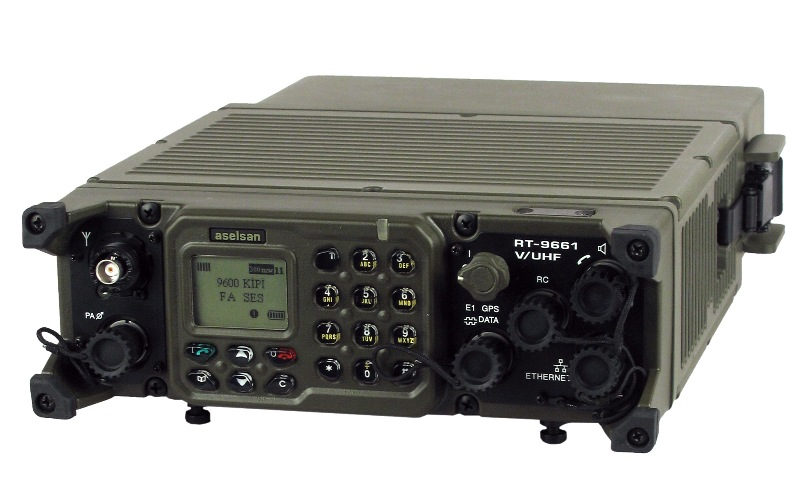
\includegraphics[scale=0.33]{radio_station}
	\caption{Радиостанция серии <<Р-181>> <<Рапсодия>>}
	\label{fig:lit_reiview:meteo:radio_station}
\end{figure}

\subsection{Автоматическая метеостанция}
\label{sub:lit_review:meteo}

Автоматическая метеостанция(АМС) это комплексный универсальный метеорологический модуль - компактное и легкое
устройство, оснащенное набором датчиков, необходимых для измерения основных метеорологических величин ~\cite{wxt530}:
\begin{itemize}
	\item направления и скорости ветра
	\item атмосферного давления
	\item температуры и относительной влажности
\end{itemize}

АМС с успехом применяется в ракетных войсках и артиллерии для определения метеорологических условий стрельбы, расчет суммарных поправок на отклонение условий стрельбы.
Модуль легко устанавливается на штатной штанге командно-штабной машине дивизиона с помощью одного винта.
Поскольку модуль не имеет движущихся частей, он надежен в эксплуатации и практически не требует обслуживания.
Используемые материалы обладают высокой устойчивостью к различным загрязнения и суровым погодным условиям.
Модуль соединяется с приемным устройством двунаправленной линией передачи.

\begin{figure}[ht]
	\centering
	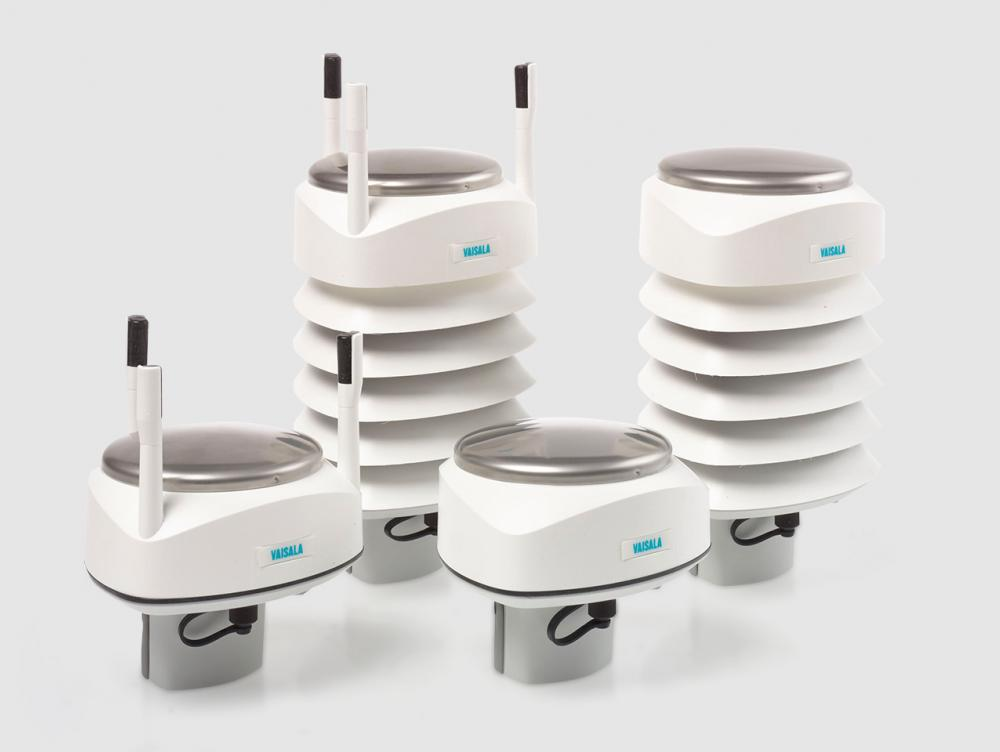
\includegraphics[scale=0.3]{meteo_station}
	\caption{Автоматическая метеостанция WXT530~\cite{wxt530}}
	\label{fig:lit_reiview:meteo:meteo_station}
\end{figure}

\subsection{Специальный принтер}
\label{sub:lit_review:spec_printer}
Специальный принтер предназначен для эксплуатации в составе мобильных вычислительных комплексов.
Может эксплуатироваться в процессе движения транспортных средств ~\cite{mp2200}.

Наиболее удобным для эксплуатации в машине КМУ является термопринтер. Термопринтеры гораздо более устойчивы к вибрациям и ударам, чем лазерные, матричные и струйные принтеры.

Корпус выполнен из металла, что обеспечивает стойкость к внешним механическим воздействиям.
Разъемы питания и интерфейсов (USB/LPT) принтера –высоконадежные «военные» байонетные металлические с металлической защитной заглушкой.
Интерфейс – высокоскоростной параллельный ECP/EPP и/или USB.

\begin{figure}[ht]
	\centering
	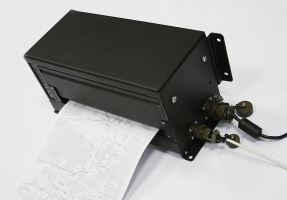
\includegraphics[scale=1.0]{printer}
	\caption{Специальный принтер МП2200~\cite{mp2200}}
	\label{fig:lit_reiview:spec_printer:printer}
\end{figure}
